\documentclass[10pt,a4paper,twocolumn]{article}

\usepackage[utf8]{inputenc}
\usepackage[T1]{fontenc}
\usepackage{newtxtext,newtxmath}
\usepackage{microtype}
\usepackage[left=1.75cm,right=1.75cm,top=1.65cm,bottom=1.85cm]{geometry}
\usepackage{graphicx}
\usepackage{booktabs}
\usepackage{tabularx}
\usepackage{array}
\usepackage{enumitem}
\usepackage[font=footnotesize,labelfont=bf]{caption}
\usepackage{placeins}
\usepackage{textcomp}
\usepackage{xcolor}
\usepackage[numbers,square,sort&compress]{natbib}
\usepackage{xurl}
\usepackage[hidelinks]{hyperref}

\emergencystretch=1.0em
\setlength{\columnsep}{0.65cm}
\setlength{\parindent}{1em}
\setlength{\parskip}{0pt}
\renewcommand{\arraystretch}{1.1}
\clubpenalty=10000
\widowpenalty=10000
\graphicspath{{figures/}}
\setlist{itemsep=2pt, topsep=4pt}
\newcolumntype{Y}{>{\raggedright\arraybackslash}X}

% Visible marker for claims that still need a citation.
\newcommand{\needsource}[1]{\textcolor{red}{[source needed: #1]}}


% --- Conference-publication-style first-page author block ---
% No supervisor email is shown where it was not supplied.
\newcommand{\studentblock}[2]{%
  \parbox[t]{0.30\textwidth}{\centering\scriptsize
    {\normalsize\bfseries #1}\\[3pt]
    \textit{Department of Computer Engineering}\\
    \textit{Faculty of Engineering}\\
    \textit{University of Peradeniya}\\
    \textit{Peradeniya, Sri Lanka}\\
    \texttt{#2}
  }%
}
\newcommand{\supervisorblock}[3]{%
  \parbox[t]{0.235\textwidth}{\centering\scriptsize
    {\small\bfseries #1}\\[3pt]
    \textit{#2}\\
    \textit{University of Peradeniya}\\
    \textit{Peradeniya, Sri Lanka}\\
    #3
  }%
}

\begin{document}
\twocolumn[{
\begin{center}
{\LARGE\bfseries Minimum IMU Devices Required and Their Placement\\[2pt]
for Walking Gait Analysis: A Literature Review\par}
\vspace{0.70cm}
\noindent
\studentblock{M. N. A. Fikry}{e21138@eng.pdn.ac.lk}
\hfill
\studentblock{W. S. S. Perera}{e21302@eng.pdn.ac.lk}
\hfill
\studentblock{D. M. E. S. Dewagedara}{e21087@eng.pdn.ac.lk}

\vspace{0.55cm}
\noindent
\supervisorblock{Roshan Godaliyadda}{Dept. of Electrical \& Electronic Eng.}{\texttt{roshang@eng.pdn.ac.lk}}
\hfill
\supervisorblock{Roshan Ragel}{Department of Computer Engineering\\\textit{Faculty of Engineering}}{\texttt{roshanr@eng.pdn.ac.lk}}
\hfill
\supervisorblock{Asanga Ratnaweera}{Department of Mechanical Engineering\\\textit{Faculty of Engineering}}{\vphantom{\texttt{mpbe@eng.pdn.ac.lk}}}
\hfill
\supervisorblock{Parakrama Ekanayake}{Dept. of Electrical \& Electronic Eng.}{\texttt{mpbe@eng.pdn.ac.lk}}
\vspace{0.55cm}
\end{center}
}]
\noindent\textbf{\textit{Abstract---}}Wearable inertial measurement units (IMUs) enable gait assessment outside controlled laboratories, but the minimum number and optimal placement of sensors depend on the measurements required. This structured narrative review critically compares body-worn IMU configurations for walking detection, gait-event timing, spatial parameters and joint kinematics. It synthesizes studies of distal, lower-limb, trunk, wrist and multi-site placements, considers classical and learning-based algorithms, and evaluates generalization to turning, slow or impaired walking, misplacement, load, footwear and varied surfaces. A single IMU can support selected walking and timing outputs and, with suitable models, some spatial or joint-angle estimates. However, results from different outputs and reference standards cannot be directly ranked, and multi-sensor configurations rarely undergo systematic sensor-removal testing. Placement and algorithm performance can also deteriorate outside straight, level walking. No universal minimum therefore follows from the reviewed evidence. Future work should determine the smallest configuration for each gait output using independent reference measurements and a controlled comparison of sensor subsets across real-world walking conditions.
\par\medskip\noindent\textbf{\textit{Index Terms---}}Inertial measurement units, gait analysis, sensor placement, minimum sensor configuration, wearable monitoring, algorithm robustness.


% =====================================================================
\section{Introduction}
\label{sec:intro}

Walking is one of the most informative things a person does every day. Small changes in how someone walks, such as slower steps, shorter strides, or a wider or more variable base, can be early signs of neurological or joint disease, and tracking them over time can show whether a treatment is working. In practice, gait is usually measured in a short, supervised test in a clinic or laboratory. That test shows what a person can do on the day and under observation, which is not always what they do in daily life \citep{carcreff2020}.

Wearable inertial measurement units (IMUs) make it possible to measure gait continuously outside the laboratory. An IMU is small and inexpensive, and records how the body segment it is attached to accelerates and rotates. The difficulty lies in deciding how many IMUs to use and where to place them. More sensors capture more of the body's movement, but they take longer to put on, must be synchronised and calibrated, and are less likely to be worn for days at a time. Fewer sensors are comfortable and practical, but at some point accuracy falls below what is useful. The places people are most willing to wear a sensor, such as the wrist and the lower back, are also the furthest from the feet, where the events that define each step take place.

This review brings together the evidence on that trade-off. It first describes what each body location can and cannot measure, then examines the algorithms that try to extract more information from fewer sensors, and finally considers the conditions under which configurations that work in the laboratory begin to fail: turning, slow or impaired walking, imperfect attachment, carried load, terrain and footwear. Throughout, the \emph{minimum configuration} is defined as the smallest set of IMUs, in number and placement, that achieves a stated accuracy for a specified gait output, population, setting and algorithm, while remaining practical for its intended use. The review asks:

\begin{enumerate}[label=\textbf{Q\arabic*.}]
  \item How many IMUs are required for each gait output?
  \item Which placements achieve the required accuracy, and under what conditions?
  \item Which algorithms reduce hardware requirements, and at what cost?
  \item What remains unresolved?
\end{enumerate}

\subsection{Problems with the current evidence}
\label{sec:problems}

Read as a whole, the literature shows several problems that recur across placements and algorithms. They are listed here and examined in detail in Sections~\ref{sec:placement}--\ref{sec:factors}.

\begin{enumerate}[label=\textbf{P\arabic*.}]
  \item \textbf{Narrow testing conditions.} Most of the smallest configurations reported so far were tested with healthy adults walking straight, on level ground and at a comfortable speed in a laboratory. Turns, stairs, slopes, postural transitions and slow or impaired walking are tested far less often.
  \item \textbf{Sensor sets chosen in advance.} Multi-sensor studies usually fix their sensor set before data collection and rarely ask which sensors could be removed without losing accuracy, so the true minimum is seldom measured directly.
    \item \textbf{Convenience may conflict with output-specific accuracy.} Wrist and lower-back placements can be practical for prolonged wear, but their reliability depends on the parameter and activity; the wrist, in particular, can be confounded by independent arm motion.
  \item \textbf{Algorithms tested in limited settings.} Learning-based models and cross-location transfer can reduce the number of sensors, but they need large labelled datasets, and most have been tested only on straight walking or checked against the teacher sensor rather than an independent reference.
  \item \textbf{Real-world factors studied in isolation.} Self-attachment, sensor shift during wear, carried load, terrain and footwear change the signal, but each has been studied on its own, and their effect on the minimum number of sensors has not been tested.
  \item \textbf{Results that are hard to compare.} Studies use different reference systems, event-matching windows and accuracy metrics, and group averages can hide large errors on individual strides.
\end{enumerate}

\subsection{Scope and structure}

The review covers body-worn IMUs during walking, including turns, stairs and transitions. Insole-based systems are mentioned only as reference or comparison devices, and upper-limb tasks are excluded. Military benchmark exercises, such as loaded marches, load-carriage time trials and agility runs, are included as an applied case. They combine in one standardised task the conditions that most challenge a small sensor set: external load, boots, gradients, long duration and non-cyclic manoeuvres. They therefore show whether configurations established in level walking still hold under demanding conditions (Sections~\ref{sec:placement-military}, \ref{sec:factors-military} and \ref{sec:disc-military}). Running is otherwise outside the scope; running and agility results are reported only where they form part of these military tasks \citep{fain2024a,fain2024b,papadakis2023,kessels2021}. Primary sources were organised by gait output, sensor placement, IMU count, algorithm, participant group, walking task, validation reference and reported accuracy metric. Instrumented insoles and pressure-only systems were treated as comparison devices rather than qualifying body-worn IMU configurations. For each result, the synthesis distinguishes measurement \emph{capability}---a configuration was shown to estimate an output---from a verified \emph{minimum}, where fewer sensors were directly compared under an explicit accuracy criterion.

\paragraph{Search and selection.} Studies were identified through searches of IEEE Xplore, PubMed, Scopus, Web of Science, ScienceDirect and Google Scholar, last run on 7 October 2026. Search strings combined sensor terms (``inertial measurement unit'', IMU, ``inertial sensor'', accelerometer, gyroscope) with gait terms (gait, walking, kinematics, posture, balance) and one topic group at a time: signal processing and feature extraction, sensor fusion and orientation estimation, machine and deep learning, terrain and walking surface (uneven, slope, stairs), and footwear (shoe, boot, barefoot). Results were limited to peer-reviewed experimental work published between 2020 and 2026, with preference given to high-ranking journals. Roughly 80 papers were screened against the scope above, and 50 were retained. Six of these predate 2020 and were kept because no recent equivalent was found. One is a standard gait textbook, used for the definition of the gait cycle \citep{perry2010}. Two supply clinical reference values: the meaningful change in gait speed \citep{perera2006} and the step-width difference in cerebellar ataxia \citep{buckley2018}. The other three are the only reviewed studies of their kind: foot-derived labels training a torso model \citep{koroglu2018}, lumbar-IMU detection of sit-to-stand transitions \citep{pham2018}, and shank-based event detection in urban outdoor walking \citep{storm2016}.

Section~\ref{sec:background} introduces gait outputs, sensing errors and reference standards. Section~\ref{sec:placement} examines configurations by placement, Section~\ref{sec:algorithms} reviews algorithms, Section~\ref{sec:factors} considers movement complexity and real-world conditions, Section~\ref{sec:gaps} sets out the research gaps, Section~\ref{sec:discussion} synthesizes the implications for practice and experimental design, and Section~\ref{sec:conclusion} concludes the review.

% =====================================================================
\section{Background}
\label{sec:background}

\subsection{Describing walking gait}

A gait cycle comprises a stride, from initial contact of one foot to its next initial contact, divided into stance and swing, with swing beginning at toe-off \citep{perry2010}. Gait outputs impose different sensor requirements:

\begin{itemize}
  \item \textbf{Temporal:} gait events, stride time, stance and swing duration, cadence, variability and left--right asymmetry.
  \item \textbf{Spatial:} stride length, walking speed and step width. Placement affects accuracy; shank sensors may suit event detection, while foot sensors may better capture step width and asymmetry \citep{voisard2024}.
  \item \textbf{Rotational:} joint angles \citep{niswander2020,wang2025l} and three-dimensional segment rotations. The helical axis describes relative segment motion as rotation about an instantaneous axis, and has been measured during walking with two IMUs on the femur and tibia \citep{nishizawa2026}.
\end{itemize}

Thus, event timing may be estimated with one sensor, whereas direct joint-motion measurement generally requires sensors on both connected segments. Learned models can reduce this requirement, with ankle-angle errors of approximately 4\textdegree{} reported using one heel IMU \citep{wang2025l}.


\begin{table*}[!t]
 \centering\small
 \caption{Gait outcome classes and the information they require. Counts describe reported approaches, not universal minima.}
 \label{tab:outputs}
 \begin{tabularx}{\linewidth}{@{}p{2.25cm}YY@{}}
 \toprule
 Output class & Example measurements & Sensor-information requirement \\
 \midrule
 Activity / temporal & Walking bouts, initial contact, toe-off, cadence, stride time & Repeating local or trunk motion; one IMU has been demonstrated for selected outputs \citep{prigent2023,romijnders2022}. \\
 Spatial & Speed, stride length, step width & Trajectory/velocity estimation or learned inference; lateral width remains more challenging \citep{zadka2024,wang2025h}. \\
 Rotational / joint & Segment orientation, knee/ankle angles, axial rotation & Adjacent-segment orientation for direct relative angles; one-sensor learned estimation is possible for selected targets \citep{niswander2020,wang2025l}. \\
 \bottomrule
 \end{tabularx}
\end{table*}

\subsection{IMU sensing and error sources}

An IMU combines a three-axis accelerometer and gyroscope, sometimes with a magnetometer. It measures acceleration and angular velocity in its own coordinate frame, requiring integration and additional assumptions to estimate position and orientation. Key error sources include:

\begin{itemize}
  \item \textbf{Drift:} integration errors accumulate over time. Foot-worn sensors use zero-velocity updates during stance; residual distance error can be approximately 1\% \citep{ruizruiz2024}. Fixed stance-detection thresholds may fail during activities such as stair negotiation \citep{wagstaff2020}.
  \item \textbf{Misalignment:} sensor axes rarely match anatomical axes. Orientation-invariant methods and deep learning can reduce sensitivity to misalignment \citep{guimaraes2021,romijnders2022}.
  \item \textbf{Attachment position:} different placements can produce similar average stride-length errors but substantially different single-stride errors and variability estimates \citep{kuderle2022}.
  \item \textbf{Soft-tissue artefact:} skin and muscle movement relative to bone introduces measurement errors; placement over bony landmarks may help \citep{scalera2021,nishizawa2026}.
  \item \textbf{Synchronisation:} multiple sensors require temporal alignment, achieved through shared computer clocks or hardware pulses \citep{nishizawa2026,anderson2025}.
\end{itemize}

\subsection{Reference standards and evaluation}

Laboratory references include optical motion capture, force plates and instrumented walkways \citep{romijnders2021,lewin2022,anderson2025}. Although accurate, these systems capture short, controlled assessments rather than everyday performance. Real-world validation therefore requires wearable references. For example, Mobilise-D, a research consortium that validates measures of real-world mobility from wearable devices, tested a lower-back device against a multi-sensor wearable reference during 2.5 hours of daily activity \citep{mico2023}.

Reference labels and evaluation methods also affect reported accuracy. Foot dragging during 180\textdegree{} turns can make stride boundaries ambiguous, requiring manual correction \citep{romijnders2021}. Event-matching windows vary from $\pm$16 to $\pm$250\,ms \citep{anderson2025}, while F1 scores can differ depending on whether results are aggregated per test or cross-validation fold \citep{kuderle2024}. Group-level agreement may also conceal individual errors \citep{lewin2023}. Furthermore, stride-time variability measured using waist and ankle IMUs showed fair-to-good reliability (ICC 0.47--0.66), compared with excellent reliability for force plates (ICC 0.90) \citep{rantalainen2020}.

Accordingly, this review reports each sensor configuration alongside its accuracy, reference system and testing conditions to support meaningful comparisons.

% =====================================================================
\section{Placement-by-Placement Analysis of IMU-Based Gait Assessment}
\label{sec:placement}

IMU placement influences the gait parameters that can be measured, their accuracy, and the complexity of the required processing algorithms. Although distal, lower-limb, proximal, and wrist placements have demonstrated effectiveness for specific gait outcomes, their performance cannot be directly generalized across different measurements or walking conditions. Therefore, identifying the minimum sensor configuration requires evaluating both anatomical placement and the intended gait parameters.

\begin{figure}[htbp]
  \centering
  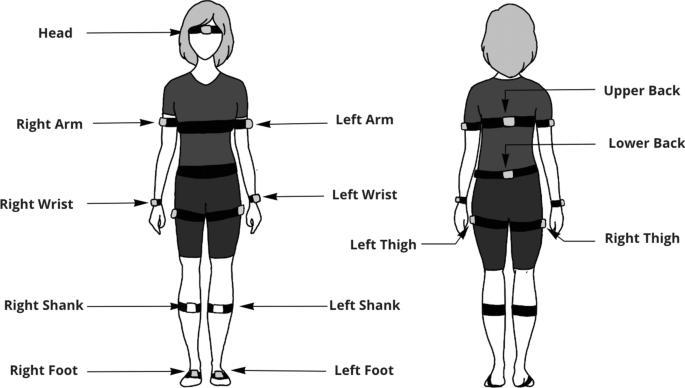
\includegraphics[width=0.7\linewidth]{fig1_placements.jpg}
  \caption{Common anatomical locations of body-worn IMUs for gait analysis. Illustrative overview, not a minimum-sensor prescription.}
  \label{fig:placements}
\end{figure}

\subsection{Distal placements: foot and insole}

Foot-mounted IMUs are particularly suitable for gait-event detection and spatiotemporal measurements because they capture movement directly associated with foot contact and swing. \citet{guimaraes2021} proposed an orientation-invariant method for estimating gait parameters using foot-worn inertial sensors. Validation against optical motion capture reported a gait-speed estimation error of $-3.1 \pm 9.2$\,cm/s, reduced in variability to $-3.4 \pm 6.9$\,cm/s when turning strides were excluded. These results demonstrate that orientation-independent processing can reduce dependence on precise sensor alignment, although performance remains affected by complex walking trajectories.

Similarly, \citet{prigent2023} demonstrated that a single foot-mounted IMU could detect walking during free-living activities in 18 participants, achieving 98\% sensitivity and 91\% specificity against a multisensor reference system. However, walking-bout detection does not establish equivalent accuracy for individual gait events or spatial measurements.

In contrast, \citet{loukovitis2021} evaluated the test--retest repeatability of 28 gait variables from IMU-embedded PODOSmart insoles in 22 healthy male participants; because the measuring device is an insole, this evidence lies outside the body-worn scope of this review. Their reported test--retest ICC values ranged from 0.802 to 0.997, demonstrating good-to-excellent repeatability. Unlike \citet{guimaraes2021}, who examined validity against motion capture, this study primarily assessed measurement consistency.

Collectively, these studies support distal placement for walking detection and spatiotemporal assessment. Nevertheless, their different validation objectives prevent a definitive ranking of foot-mounted and insole-integrated IMUs. Furthermore, distal sensors cannot independently capture proximal joint rotations, and spatial estimates remain dependent on drift correction and processing assumptions.

\subsection{Lower-limb placements: shank and thigh}

Shank- and thigh-mounted IMUs provide segment-specific motion information for gait-event detection and lower-limb kinematics. \citet{niswander2020} evaluated 11 sensor locations in seven participants performing the Timed Up and Go test. Comparisons against optical motion capture demonstrated that joint-angle bias and root-mean-square error varied with anatomical placement, target joint, and functional movement. However, the small sample limits generalization across populations and walking conditions.

\citet{kahlon2023} examined acceleration and angular-velocity signals from bilateral shank and thigh IMUs in 30 adolescents under different walking speeds and treadmill/overground conditions. Superior--inferior shank acceleration and mediolateral shank angular velocity demonstrated comparatively stable signal characteristics. However, signal consistency does not necessarily establish joint-angle accuracy.

\citet{salminen2024} evaluated a shank-angular-velocity method using 24,519 strides across nine scenarios, demonstrating accurate detection of several gait events, although heel-rise detection remained less accurate.

Together, these studies indicate that shank placement is promising for gait-event analysis, whereas optimal joint-kinematic placement remains measurement-dependent. They do not establish a universally optimal lower-limb configuration.

\begin{figure}[htbp]
  \centering
  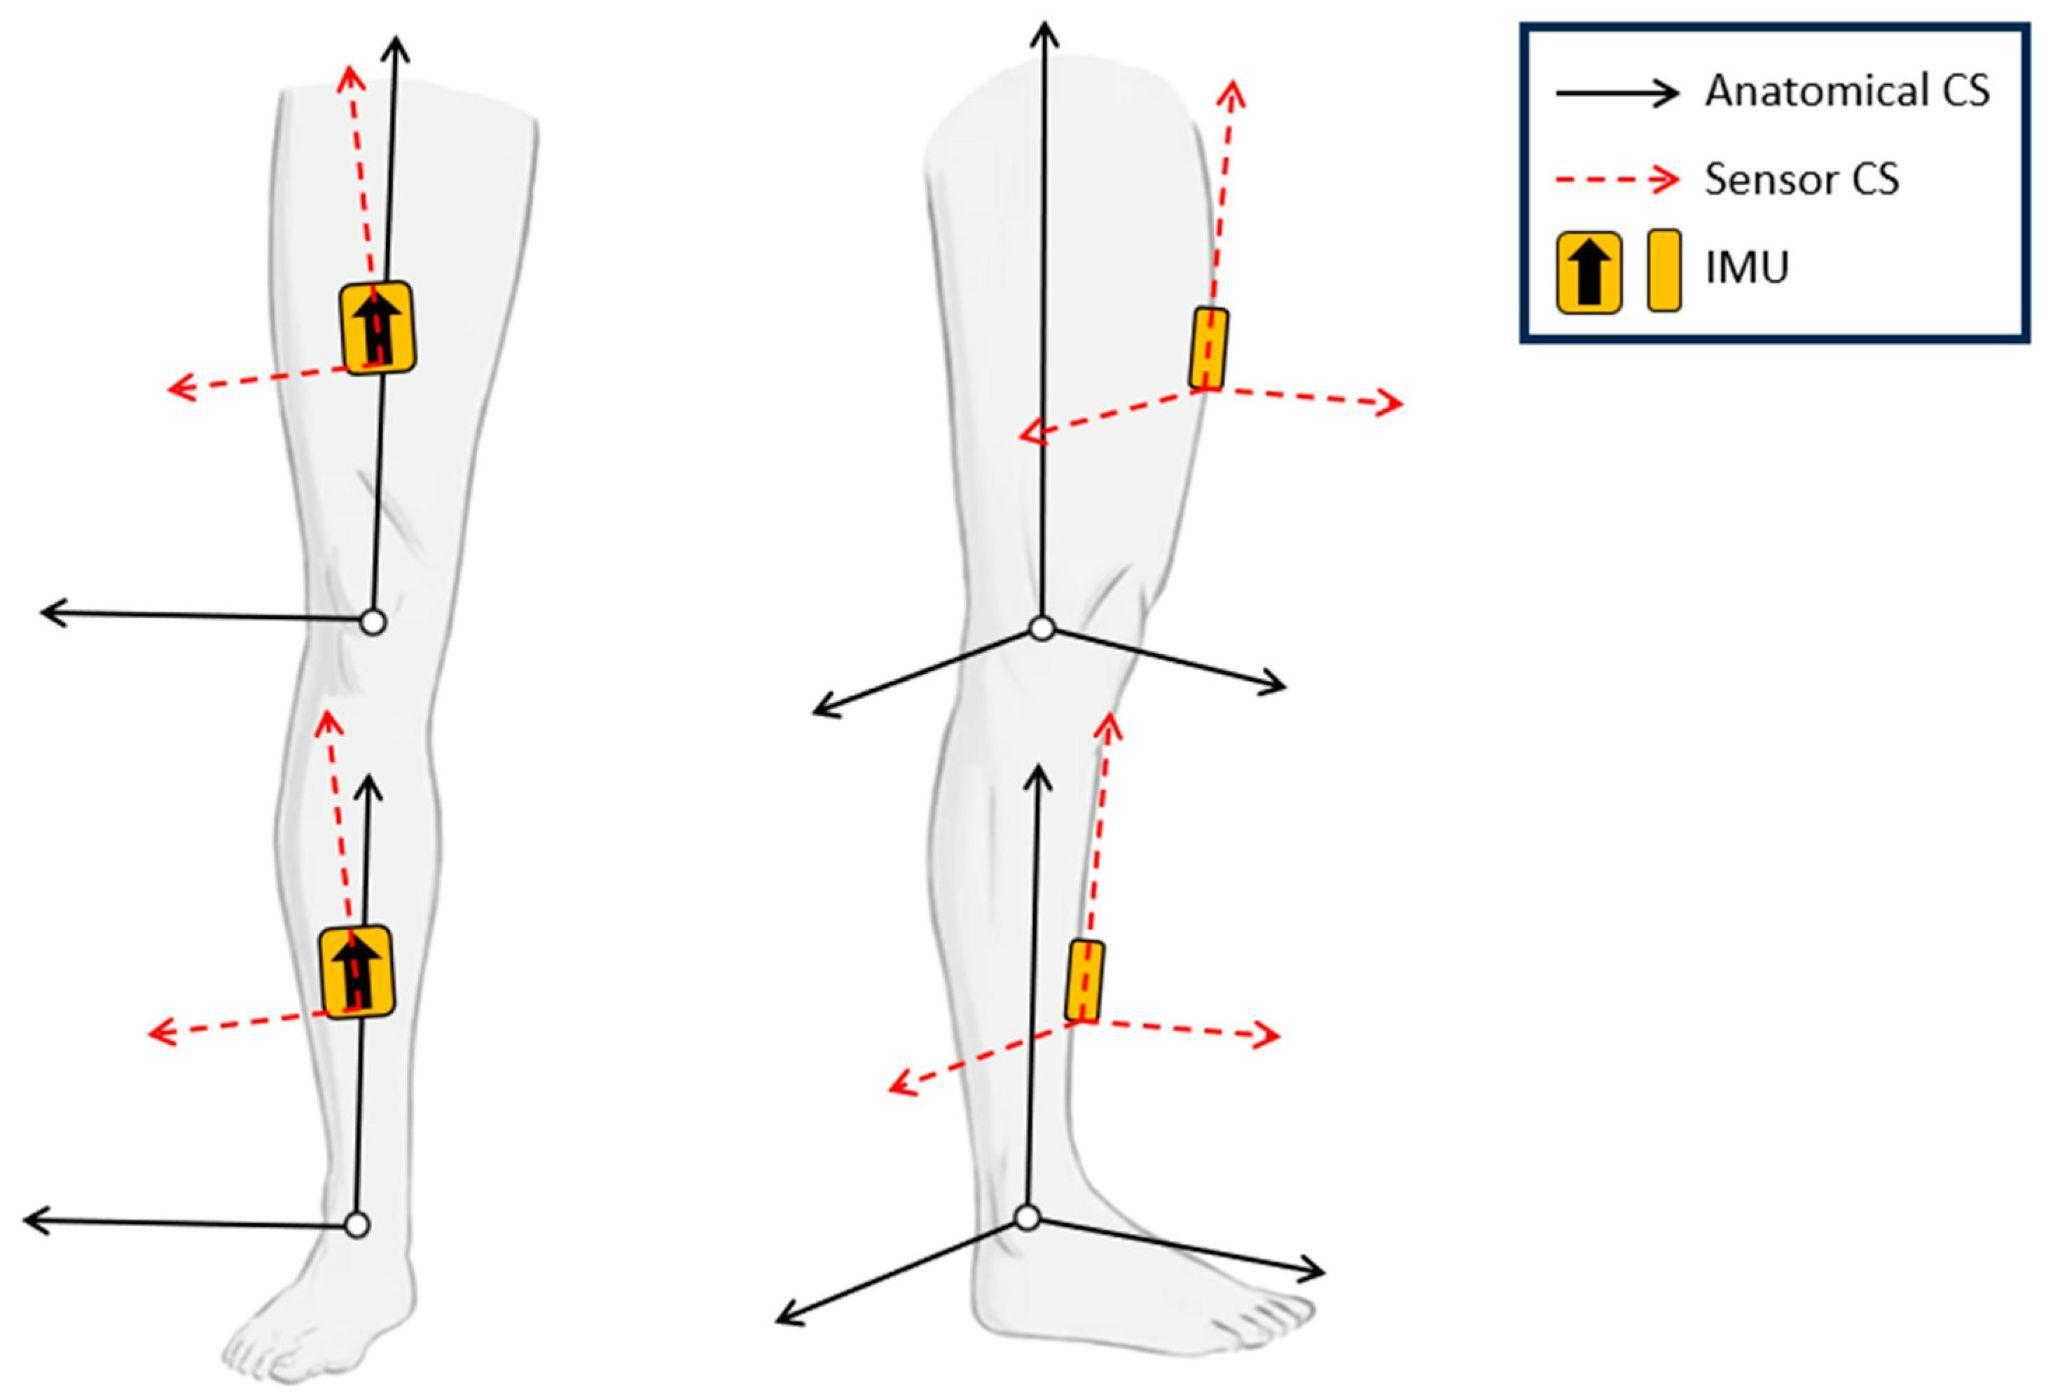
\includegraphics[width=0.8\linewidth]{fig2_misalignment.jpg}
  \caption{Conceptual illustration of sensor-to-segment misalignment and attachment movement affecting lower-limb IMU measurements.}
  \label{fig:misalignment}
\end{figure}

\subsection{Proximal placements: lower back, waist and chest}

Proximal IMUs are frequently used for global gait assessment because they capture trunk movement and are practical for long-duration monitoring. \citet{rantalainen2020} compared waist- and ankle-mounted IMUs in 27 older adults. Although both locations showed excellent reliability for mean stride duration, waist placement produced higher reliability for stride-duration variability (ICC = 0.66) than ankle placement (ICC = 0.47). This demonstrates that optimal placement depends on the selected gait outcome.

\citet{mico2023} evaluated lower-back IMU algorithms in 108 participants across six healthy and clinical cohorts. Walking-sequence detection, cadence, and initial-contact estimates showed generally strong performance. However, shorter walking bouts, speeds below 0.5\,m/s, and severe gait impairment reduced the accuracy of certain outcomes, particularly stride length.

\citet{lueken2021} investigated pendant-based step-length estimation in ten healthy participants, reporting relative errors below 10\% at walking speeds of 2--4\,km/h. Unlike waist-fixed sensors, pendant motion introduces different mechanical and modeling considerations.

These studies support proximal placements for global mobility measurements but show that accuracy is outcome-, algorithm-, and population-dependent. They provide limited direct evidence for reconstructing independent knee and ankle kinematics.


\begin{figure}[htbp]
 \centering
 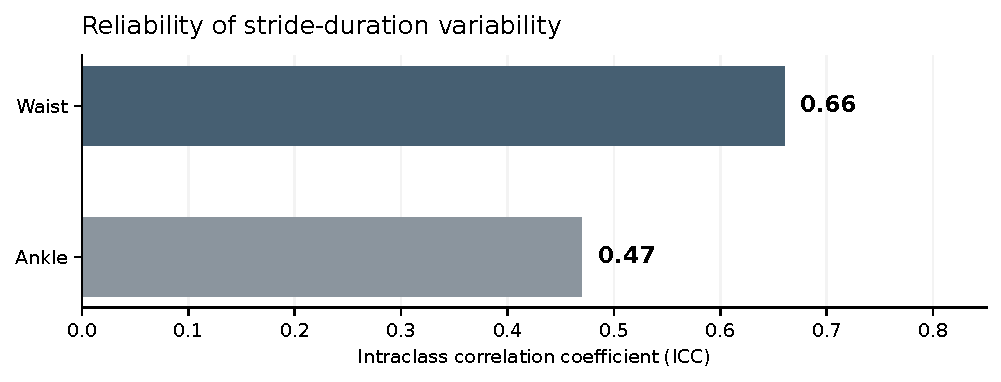
\includegraphics[width=0.81\linewidth]{fig4_waist_ankle_icc.pdf}
 \caption{Within-study comparison of stride-duration variability reliability at waist and ankle placements. ICC values reported by Rantalainen et al. \citep{rantalainen2020}; reliability is not equivalent to absolute measurement validity.}
 \label{fig:waist-icc}
\end{figure}

Figure~\ref{fig:waist-icc} makes the placement difference explicit for the \emph{same} outcome and study. The waist ICC exceeds the ankle ICC (0.66 versus 0.47), but the comparison concerns repeatability in older adults and does not identify an optimal location for gait events, step width or joint-angle estimation.

\subsection{Upper-extremity placement: wrist}

Wrist-mounted IMUs offer convenient long-term monitoring but introduce uncertainty because arm movements are not exclusively associated with walking. \citet{brand2022} evaluated wrist-based gait detection in 30 older adults, including participants with Parkinson's disease. Their deep convolutional neural network achieved AUC values of 0.94 and 0.89 for older-adult and Parkinson's groups, respectively, although precision--recall performance was lower.

\citet{kluge2024} examined 83 participants across six cohorts, reporting wrist-based walking-detection sensitivities of 0.55--0.81, compared with 0.71--0.91 for lower-back algorithms.

Together, these findings indicate that wrist placement supports ambulatory activity detection but generally offers less reliable walking identification than lower-back placement. Its suitability for detailed lower-limb kinematics remains insufficiently demonstrated.

\subsection{Multi-site IMU configurations}

Multi-site configurations combine information from several body segments, enabling assessment of bilateral movement, coordination, and complex gait characteristics. \citet{carcreff2020} employed five synchronized IMUs on the chest, thighs, and shanks in 15 children with cerebral palsy and 14 typically developing children. Comparing laboratory assessments with three days of daily-life monitoring, they identified substantial differences in multiple gait characteristics between controlled and natural environments.

Similarly, \citet{lin2023} employed ten IMUs to distinguish early Parkinson's disease from essential tremor using gait and postural-transition features. Their machine-learning approach achieved 84\% cross-validation accuracy but only 75.8\% accuracy on independent test data, indicating limitations in generalization.

Although these studies demonstrate the value of multisite information, neither systematically establishes whether every sensor is necessary. Additional IMUs also increase synchronization, calibration, attachment, and processing requirements.

\paragraph{Cross-placement synthesis.} The evidence indicates that optimal sensor configurations are parameter-dependent rather than universally defined. Distal sensors support foot events, shank sensors provide useful gait-phase signals, and proximal sensors enable global mobility monitoring. Multi-site systems capture broader movement information, but their additional value over reduced configurations is not consistently quantified (Table~\ref{tab:placement}). Therefore, a remaining research opportunity is to determine the smallest sensor configuration that maintains predefined measurement accuracy across multiple gait parameters, participant groups, and walking conditions.

\begin{figure}[htbp]
  \centering
  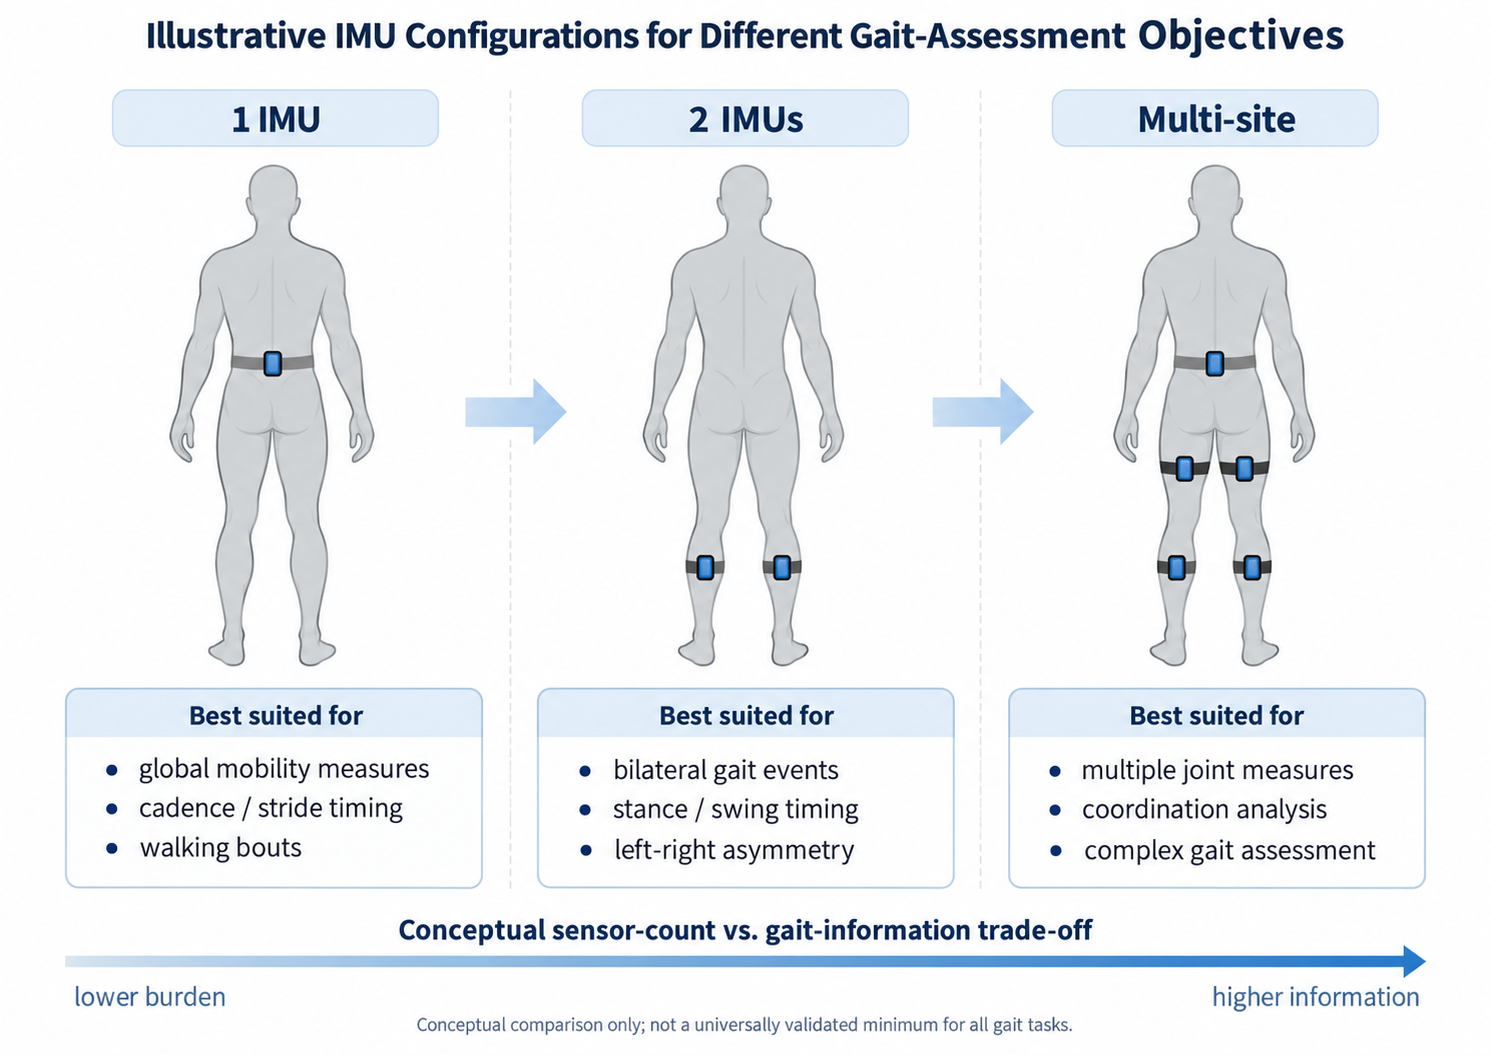
\includegraphics[width=0.75\linewidth]{fig3_configurations.png}
  \caption{Illustrative IMU configurations for different gait-analysis objectives. A single foot-mounted IMU has been used for walking-bout detection \citep{prigent2023}, whereas waist/lower-back IMUs support selected temporal and global gait measurements \citep{mico2023,rantalainen2020}. The configurations are examples of demonstrated capabilities, not universally validated minimum sensor requirements.}
  
  \label{fig:configurations}
\end{figure}

\begin{table*}[!t]
  \centering
  \caption{Summary of placement evidence and its implication for the minimum IMU configuration.}
  \label{tab:placement}
  \small
  \begin{tabularx}{\linewidth}{@{}p{2.2cm}YYY@{}}
    \toprule
    Placement & Main evidence & Limitations & Minimum-IMU implication \\
    \midrule
    Foot & \citet{guimaraes2021}; \citet{prigent2023}: walking detection, spatiotemporal estimates & Joint-specific information and spatial drift & One sensor can support some walking outcomes \\
    \addlinespace
    Shank/thigh & \citet{niswander2020}; \citet{kahlon2023}; \citet{salminen2024}: joint accuracy, robust signals, gait phases & Placement dependence and joint-specific errors & Minimum depends on gait event versus joint kinematics \\
    \addlinespace
    Waist/lower back/chest & \citet{rantalainen2020}; \citet{mico2023}; \citet{lueken2021} (chest pendant): global gait outcomes and clinical monitoring & Slow gait, short bouts, limited joint detail & One sensor supports selected global measurements \\
    \addlinespace
    Wrist & \citet{brand2022}; \citet{kluge2024}: long-term walking detection & Confounding arm movements; lower sensitivity & Suitable for detection, not established for detailed joint kinematics \\
    \addlinespace
    Multi-site & \citet{carcreff2020}; \citet{lin2023}: multi-domain gait assessment & Complexity; sensor redundancy untested & Sensor reduction requires systematic evaluation \\
    \bottomrule
  \end{tabularx}
\end{table*}


\begin{table*}[!t]
 \centering\footnotesize
 \caption{Selected primary studies compared on evaluation design and interpretation. Distinct outcomes and metrics must not be numerically ranked against each other.}
 \label{tab:study-comparison}
 \renewcommand{\arraystretch}{1.14}
 \begin{tabularx}{\linewidth}{@{}p{2.15cm}p{1.6cm}YY@{}}
 \toprule
 Study / configuration & Target and validation & Reported result & Interpretation and limitation \\
 \midrule
 Prigent et al. \citep{prigent2023}; one foot IMU & Free-living walking bouts; multi-sensor reference & 98\% sensitivity; 91\% specificity & Demonstrates walking detection, not heel-strike or spatial validity. \\
 Romijnders et al. \citep{romijnders2022}; one shank/ankle IMU & Initial/final contact; independent test participants & Recall $\geq$92\%; precision $\geq$97\% & Strong event evidence; model and cohort dependence. \\
 Rantalainen et al. \citep{rantalainen2020}; waist/ankle & Stride-time variability; reliability analysis & ICC 0.66 versus 0.47 & Within-study reliability; not a validity test. \\
 Zadka et al. \citep{zadka2024}; lower back & Step length; reference-labelled model & RMSE 6.08\,cm & One-sensor spatial estimate; population and training matter. \\
 Lin et al. \citep{lin2023}; ten IMUs & Neurological classification; independent testing & 84\% cross-validation, 75.8\% held-out & More sensors did not establish a minimum; generalization dropped. \\
 \bottomrule
 \end{tabularx}
\end{table*}

These examples also distinguish three often-conflated forms of evidence: detection accuracy, continuous-parameter error and repeatability. They are not interchangeable. Similarly, a multi-site study may prove that a rich configuration works without establishing whether one of its devices can be removed. Thus, an output-specific minimization experiment should fix its reference system and metrics before comparing candidate sensor subsets.

\subsection{Placement in military benchmark exercises}
\label{sec:placement-military}

Military benchmark exercises, such as loaded marches, load-carriage time trials and agility runs, impose a constraint that clinical studies rarely face: sensors must coexist with boots, body armour and rucksacks. \citet{slattery2024} compared four boot-mounted IMUs and one instrumented insole with treadmill force plates in 19 Australian Army trainees walking at 5.5\,km/h with 23\,kg. All devices showed good-to-excellent agreement for linear stride-time variability (ICC $>$ 0.88), whereas agreement for non-linear measures was lower (ICC 0.57--0.92). The authors chose the boot because it would least affect a soldier's duties. \citet{fain2024b} similarly mounted the distal sensor on footwear because military boots prevent tibial placement, while \citet{feigel2026} strapped two IMUs to the distal tibia over the boots during an outdoor 6.72\,km load-carriage time trial.

Proximal placement was preferred for recognising activity type. \citet{papadakis2023} selected the waist over the arm and thigh because it produced more consistent signals, and a random-forest classifier subsequently reached 92.9\% validation accuracy, and 83.6\% on unseen test participants, for walking, uphill walking, running and jumping in 50 military participants. Where joint kinematics were required, studies relied on multi-segment systems, ranging from a foot, shank, thigh and pelvis set \citep{fain2024a} to a 17-IMU full-body suit \citep{kessels2021}.

These studies suggest that, in military testing, feasible placements are dictated by equipment as much as by accuracy. Boot and distal-tibia sites were selected for gait timing in the cited military tests; waist sensors supported activity recognition, and multi-segment sets supported the joint-kinematic analyses examined.

\FloatBarrier

% =====================================================================
\section{Algorithms That Reduce Sensor Needs}
\label{sec:algorithms}

The minimum IMU configuration required for accurate gait analysis depends just as heavily on algorithmic processing as it does on hardware placement. This section summarizes the classical baseline, then examines three recent algorithmic families that actively lower the sensor requirement: displacement-based segmentation, single-sensor deep learning, and cross-location transfer.

\subsection{Classical baseline}

Classical pipelines detect gait events by identifying peaks or threshold crossings in foot or shank angular velocity \citep{romijnders2021,ruizruiz2024}, or by matching signals against predefined templates and hidden Markov models \citep{kuderle2024}. Once events are detected, foot trajectories are reconstructed using zero-velocity updates during stance \citep{wagstaff2020}. Because these methods rely on characteristic signal shapes and rigid thresholds that fluctuate based on movement intensity, they have mostly been validated on straight-line walking with foot- and shank-worn sensors; where tested, shank peak detection stayed accurate in slalom walking but produced more missed and false events during turning \citep{romijnders2021}.

\subsection{Displacement-based segmentation}

To overcome the fragility of signal-shape thresholds, FoDiGS \citep{ruizruiz2024} replaces heuristic signatures with a deterministic kinematic rule: a step is defined strictly by a significant horizontal displacement of the foot from its previous stationary position. Relying on a zero-velocity-aided trajectory, heel strikes and toe-offs are registered when horizontal displacement crosses a fixed threshold (0.0045\,m).

By relying on estimated horizontal displacement rather than only on gyroscope peaks, FoDiGS was designed to handle atypical foot motion, including dragged steps. The reported comparison favored the displacement-based approach over signal-shape methods for the forward walking styles examined \citep{ruizruiz2024}. However, the demonstrated performance concerns the evaluated forward walking styles rather than a systematic test of complex walking conditions. Importantly, this approach changes how existing foot-IMU data are processed; it does not establish that physical sensor count can be reduced. Its performance during turns, stairs and loaded gait requires separate validation.

\subsection{Learning-based estimation from single sensors}

Machine and deep learning models actively reduce both physical sensor counts and manual feature engineering. For gait events, a convolutional network trained on data from a 157-participant cohort detected initial and final contacts from a single ankle or shank IMU in 48 held-out test participants (recall $\geq$ 92\%, precision $\geq$ 97\%), requiring minimal orientation knowledge \citep{romijnders2022}.

However, performance varies by placement. \citet{anderson2025} found that TCNs using lower-limb sensors exceeded an F1-score of 95\% during walking with only 5--10 participants for model development. Wrist-sensor models performed worse even with the full development set of 81 participants (F1 88.4\% for walking and 50.0\% for stationary and transitional movements). Their walking performance was still rising at that point, suggesting that more data would continue to improve them. Spatial parameters and joint kinematics show similar promise: XGBoost applied to a lower-back IMU estimated step length with a 6.08\,cm RMSE \citep{zadka2024}, and a heel-mounted convolutional network estimated ankle angles with a 4.13\textdegree{} RMSE \citep{wang2025l}. The shared limitation across learning-based methods is the immense need for reference-labeled training data, a requirement that is steepest for inherently noisy, comfortable placements like the wrist.

\subsection{Cross-location transfer}

To address the massive training data bottleneck, cross-location transfer leverages an accurate ``teacher'' sensor to supervise a comfortable ``student'' placement during data collection. Early models used rule-based foot labels to train proximal networks. \citet{koroglu2018} thresholded the gyroscope norm of a foot IMU to label stationary phases, using these to train a torso-IMU residual network to 93\% accuracy. More recently, \citet{kolakowski2024} compared four neural networks for translating wrist IMU signals into tibia or shoe signals; U-Net and a CNN autoencoder were most accurate, and in a single 10\,m walk, temporal parameters from CNN-autoencoder-translated signals were close to shoe-sensor values for stride duration (28\,ms difference) but less so for stance and swing (80 and 44\,ms). Algorithm-generated labeling also replaces manual video annotation; \citet{wagstaff2020} trained an LSTM zero-velocity detector using optimized classical detector labels. However, the cross-location studies remain proofs of concept: \citet{koroglu2018} and \citet{kolakowski2024} evaluated against their own teacher sensors rather than independent references (e.g., optical motion capture), and \citet{wagstaff2020}, although validated against independent position ground truth, addressed zero-velocity detection rather than transfer to another body site. Robust event-level transfer to the wrist, independently validated in unseen clinical populations, remains a critical open challenge.

\begin{table*}[!t]
 \centering\footnotesize
 \caption{Algorithmic approaches, their sensor-reduction potential and associated evidence limitations.}
 \label{tab:algorithms}
 \begin{tabularx}{\linewidth}{@{}p{2cm}p{1.75cm}YY@{}}
 \toprule
 Method & Sensor requirement & Benefit & Principal limitation \\
 \midrule
 Peak/ZUPT methods \citep{wagstaff2020,romijnders2021} & Often foot/shank IMU & Transparent signal processing; no large supervised dataset & Depends on motion signatures and reliable stationary detection. \\
 Displacement approach \citep{ruizruiz2024} & Foot IMU configuration & Handles some atypical steps without learned labels & Foot trajectory assumptions; no demonstrated sensor-count reduction. \\
 Supervised learning \citep{romijnders2022,zadka2024,wang2025l} & One IMU for selected outputs & Learns event, spatial or kinematic relationships & Independent reference labels, domain shift and unseen populations. \\
 Cross-location transfer \citep{koroglu2018,kolakowski2024} & Teacher during training; student in use & May enable more convenient deployment & Teacher agreement is not independent gait accuracy. \\
 \bottomrule
 \end{tabularx}
\end{table*}

\subsection{Summary}

Ultimately, each algorithmic family mitigates a distinct hardware or data constraint. Displacement-based segmentation can avoid a labeled training dataset for the particular foot-mounted processing approach considered, but does not establish a smaller hardware count. Learning-based methods actively reduce the physical hardware count, allowing a single device at selected shank, lower-back, or heel sites to estimate specific gait events, step-length outcomes, or ankle angles in the reported evaluations. Finally, cross-location transfer, though currently at the proof-of-concept stage, suggests that cumbersome reference sensors are only necessary during data collection to supervise a comfortable, long-term wearable. Whether these algorithmic gains remain robust beyond straight-line laboratory walking is examined in Section~\ref{sec:factors}.

\FloatBarrier

% =====================================================================
\section{Factors That Change the Minimum}
\label{sec:factors}

The smallest configurations reported in Sections~\ref{sec:placement}--\ref{sec:algorithms} were tested mainly in healthy adults walking straight at comfortable speed. Outside these conditions, a changed signal does not automatically mean more sensors are needed: algorithms correct poor inference, whereas additional IMUs add physically independent information. A configuration is treated here as sufficient only when its error is small relative to clinically relevant differences, about 0.05--0.10\,m/s for gait speed \citep{perera2006}, although no agreed threshold exists for event timing or step width.


\subsection{Non-cyclical movement}
\label{sec:noncyclical}

Turns, transitions, and gait initiation challenge the periodic-signal assumptions underlying many gait-event detectors. In a study of 121 older adults with and without Parkinson's disease, \citet{anderson2025} evaluated single-location temporal convolutional networks across straight walking, 180\textdegree{} turns, and stationary/transitional movements. The published abstract identifies the dorsal foot as the highest-performing sensor location, with F1 scores of 99.3\%, 96.7\%, and 88.4\%, respectively, and the wrist as the lowest-performing location, with corresponding scores of 88.4\%, 72.3\%, and 50.0\%. These values represent the highest and lowest location-specific performances across the tested sensor sites, rather than cross-study comparisons. The results show that sensor placement and movement complexity jointly influence stride-segmentation performance. However, they do not establish that increasing the number of IMUs would resolve these limitations.

Algorithm choice also matters. Foot strapdown integration outperformed lumbar pendulum models for spatial parameters during straight walking but not during continuous turning \citep{kvist2024}, although both algorithm and placement changed simultaneously. Conversely, one shank IMU reconstructed per-stride heading change with a median error of 0.7\textdegree{} (IQR $-0.2$ to 1.7\textdegree{}) \citep{uchitomi2022}, but only in 12 healthy young adults. Evidence for postural transitions remains limited: one lumbar IMU detected sit-to-stand and stand-to-sit movements with 82--85\% accuracy in Parkinson's disease and older adults, but only 47\% in participants with dyskinesia \citep{pham2018}. FoDiGS was validated on forward walking styles \citep{ruizruiz2024}, while direct, outcome-matched comparisons of reduced sensor configurations during postural transitions remain limited.

\begin{figure}[htbp]
	\centering
	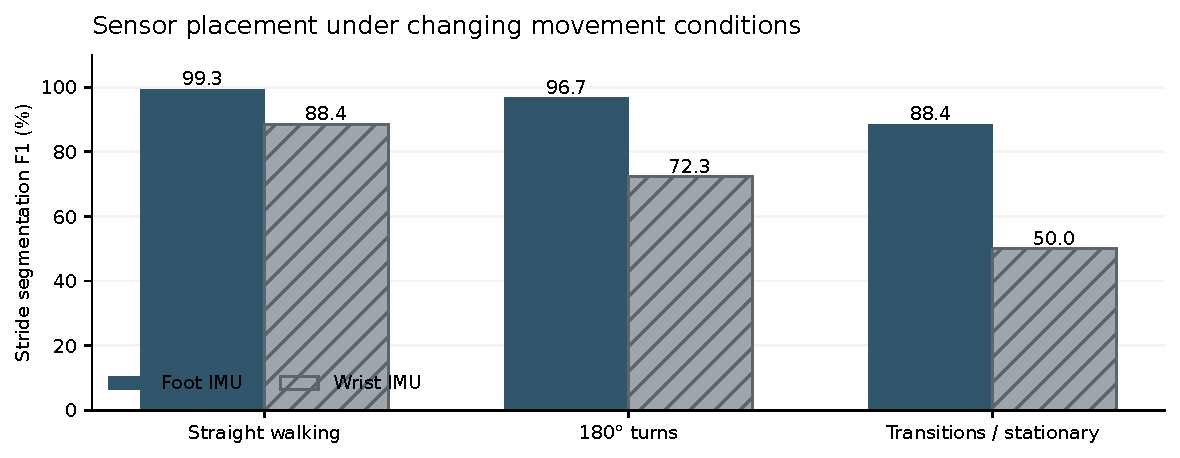
\includegraphics[width=0.96\linewidth]{fig5_foot_wrist_f1.pdf}
	\caption{Stride-segmentation F1 scores of the highest-performing dorsal-foot and lowest-performing wrist sensor locations across walking, 180\textdegree{} turns, and stationary/transitional movements. Values reported by \citet{anderson2025}. This is a sensor-placement comparison, not a sensor-count comparison.}
	\label{fig:foot-wrist}
\end{figure}

Figure~\ref{fig:foot-wrist} illustrates the differences in performance between the dorsal-foot and wrist locations. The dorsal-foot sensor achieved higher F1 scores across all three movement conditions, with the largest difference observed during stationary/transitional movements (88.4\% versus 50.0\%). This comparison highlights the importance of evaluating sensor placement under different movement conditions. However, because each result was obtained using a single-location model, the findings cannot determine whether adding sensors would improve performance.


\subsection{Pathological and slow walkers}

Pathology alters both gait and its signal, but higher error alone does not justify more hardware. Using two foot-dorsum IMUs, \citet{voisard2024} reported gait-event F1 scores of 100\%, 99.4\% and 96.3\% in healthy, multiple-sclerosis and post-stroke cohorts, with median timing error rising from 8 to 18 and 26\,ms; the patient groups walked at only 0.23--0.28\,m/s. A convolutional model developed on a 157-participant cohort (61 for training) and tested on 48 unseen participants, including Parkinson's, multiple-sclerosis and stroke cohorts, achieved recall $\geq$92\% and precision $\geq$97\% from a single shank or ankle IMU \citep{romijnders2022}, suggesting that representative training can preserve a one-sensor minimum for temporal events. Slow gait strains proximal placements more: lower-back stride-length error fell below 20\% only above 0.5\,m/s \citep{mico2023}. Step width is less forgiving still. Pelvis and bilateral-shank IMUs gave 3.3\,cm MAE during over-ground walking in spinocerebellar ataxia \citep{wang2025h}, and in healthy young men an insole--waist pair gave 40.0\,mm versus 45.4\,mm for the best single insole and 49.7\,mm for the waist, the best single body-worn sensor, without statistical comparison \citep{fukamachi2026}. Both errors approach the $\sim$6\,cm mean difference between ataxic and healthy step width \citep{buckley2018}, so whether any reduced configuration is clinically sufficient remains unresolved.

\subsection{Misplacement and shift}

The placements in Section~\ref{sec:placement} describe anatomical regions, not exact attachments. Across six foot positions in 14 healthy adults, mean stride-length error stayed below 2\,cm, but single-stride errors differed greatly, with heel-sensor outliers near 60\,cm \citep{kuderle2022}. Functional calibration reduced the shank inter-placement RMS difference in angular excursion from 15\textdegree{} to 1.5\textdegree, but gave no significant improvement at the pelvis, could worsen thigh estimates and was assessed between sensors rather than against an optical reference \citep{mihy2026}. Self-placed tibial sensors were also less repeatable than researcher-placed ones (ICC 0.55 versus 0.85) \citep{ruder2022}. A minimum configuration should therefore specify its attachment and calibration protocol, not only its sensor count. Sensor slippage during prolonged wear remains largely unquantified.


\begin{figure}[htbp]
 \centering
 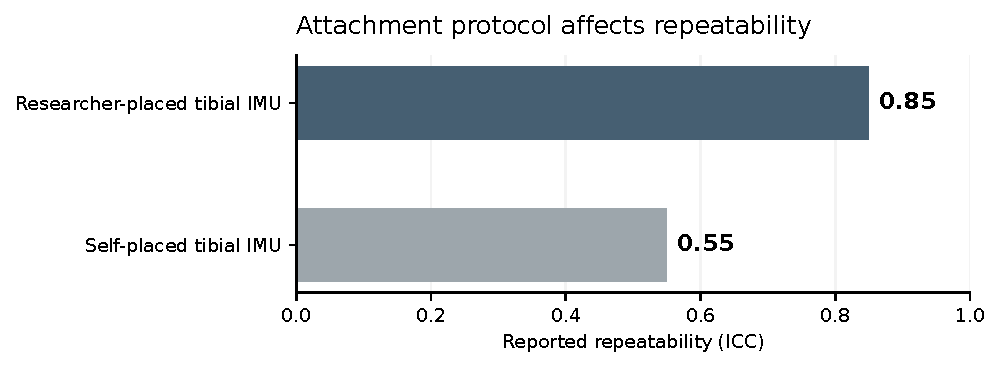
\includegraphics[width=0.80\linewidth]{fig6_self_placement_icc.pdf}
 \caption{Repeatability comparison for researcher-placed versus self-placed tibial IMUs (ICC 0.85 versus 0.55), as reported by Ruder et al. \citep{ruder2022}. Results are configuration- and study-specific.}
 \label{fig:attachment}
\end{figure}

The attachment comparison in Figure~\ref{fig:attachment} emphasizes that a nominally identical one-sensor configuration can perform differently depending on who mounts it. Protocol robustness therefore belongs in the definition of a deployable minimum, rather than being treated as a minor operational detail.

\subsection{Load, gradient and duration in military benchmark exercises}
\label{sec:factors-military}

Military benchmark exercises combine factors that clinical studies examine separately. Load alters the signal itself. In 20 adults walking and running with a 23\,kg weighted vest, load reduced peak foot and pelvis accelerations. The signal attenuation between the foot and pelvis sensors rose for each step, but fell when summed over a kilometre \citep{fain2024b}. Load and gradient also challenge kinematic estimation. A foot, shank, thigh and pelvis IMU set estimated hip and knee range of motion during walking with no significant mean difference from motion capture, although RMSE remained 12.6--18.5\textdegree; it failed during running, and it detected only a grade effect on the knee waveform and missed the other load- and grade-induced changes identified by motion capture \citep{fain2024a}. Duration matters over long events: in 14 military personnel completing a 6.72\,km time trial with 25\,kg rucksacks, the gait-variability exponent DFA-$\alpha$ fell significantly from the first to the final third of the event \citep{feigel2026}. Non-cyclic benchmark tasks extend the deficit described in Section~\ref{sec:noncyclical}. In a 32.5\,m agility run with five flags and five hurdles, adding 15.6 and 31.2\,kg increased completion time from 11.78 to 12.32 and 13.08\,s in ten participants, although the IMU-based kinematics were analysed for only one of them \citep{kessels2021}, and instrumented turning tasks, including the modified Illinois Agility Test, together discriminated mild traumatic brain injury with high accuracy (AUC 0.92; modified Illinois Agility Test alone, 0.78) in civilian adults \citep{fino2025}. None of these studies compared sensor counts under load, so whether minimum configurations derived from unloaded walking hold during military testing remains unknown.

\subsection{Footwear and walking surface}

Footwear and walking surface change both gait and how a sensor couples to the body, yet each has been tested almost only in isolation. Shoelace-mounted IMUs matched laboratory group-level orthotic effects for most variables but agreed on the direction of individual change in only 40--70\% of participants \citep{lewin2023}. By contrast, one shank IMU measured shank-to-vertical angle within 1\textdegree{} (ICC $>$ 0.9) across heel-wedge conditions \citep{dejong2021}. Footwear sensitivity therefore depends on whether the sensor is coupled to the shoe or to the body, and on the target metric. Shoe parameters beyond orthoses and heel height are largely untested: the only multi-IMU study varying heel and platform height is a three-participant preprint without a reference system \citep{meghapathirana2024}. Surface effects appear parameter-specific. Shank-based event detection stayed accurate in urban outdoor walking \citep{storm2016}, whereas nine event-detection algorithms lost performance on sloped terrains relative to flat ground \citep{trigo2025}. None of the reviewed studies varied footwear, surface and sensor configuration together.


\subsection{Cross-condition synthesis}
\label{sec:condition-synthesis}

The studies in this section do not all report the same outcome or accuracy metric, so they cannot be pooled into a single performance ranking. Nevertheless, they identify recurring, distinct reasons why a minimum estimated on level walking may not transfer to other tasks (Table~\ref{tab:conditions}). For turns and pathological gait, an algorithm can fail because expected movement signatures change; for attachment variation, the recorded signal changes even when the intended body segment is unchanged. Load and footwear can also alter the movement itself. Therefore, degraded performance must first be attributed to missing information, model mismatch or attachment error before concluding that additional sensors are required.

\begin{table*}[!t]
 \centering\footnotesize
 \caption{Cross-condition synthesis of threats to minimal IMU configurations.}
 \label{tab:conditions}
 \begin{tabularx}{\linewidth}{@{}p{2.15cm}YY@{}}
 \toprule
 Condition & Evidence of challenge & Implication for a minimum configuration \\
 \midrule
 Turns / transitions & Lower wrist F1 during transitions \citep{anderson2025}; shank peak detection misses events in turns \citep{romijnders2021}. & Retest by task; use the same reference and event matching rule. \\
 Slow / impaired gait & Lower-back stride length deteriorates below roughly 0.5\,m/s \citep{mico2023}; pathology alters timing errors \citep{voisard2024}. & Include participant diversity, shorter bouts and slow speeds. \\
 Attachment shift & Self-placement ICC 0.55 vs research placement 0.85 \citep{ruder2022}; foot location affects outliers \citep{kuderle2022}. & Compare calibrated and repeat attachments, not just nominal sites. \\
 Load / gradient & Missed grade/load kinematic changes \citep{fain2024a}; field drift over duration \citep{feigel2026}. & Validate during load and prolonged walking against independent reference. \\
 Footwear / surface & Individual orthotic responses may disagree \citep{lewin2023}; slopes reduce event-detector performance \citep{trigo2025}. & Hold footwear/surface conditions explicit when assessing subsets. \\
 \bottomrule
 \end{tabularx}
\end{table*}

\FloatBarrier

% =====================================================================
\section{Research Gaps}
\label{sec:gaps}

Across Sections~\ref{sec:placement}--\ref{sec:factors}, the evidence converges on one overarching gap: none of the reviewed studies determined the smallest set of body-worn IMUs that still measures gait to a stated accuracy across the terrains and tasks people actually encounter. The smallest configurations reported so far were derived mostly from straight, level walking in the laboratory, and studies fixed their sensor sets in advance rather than testing which sensors could be removed. Closing this gap requires three strands to be addressed together: optimising sensor placement, optimising the algorithms that extract gait from fewer sensors, and accounting for the real-world obstructions that degrade both. Military benchmark exercises, which combine load, gradient, long duration and non-cyclic movement, provide a demanding and standardised test bed for all three.

\subsection{Optimal placement across terrains and tasks}

Placement evidence is parameter-specific: foot and shank sensors give the most accurate gait events, proximal sensors support global mobility measures, and wrist sensors are weakest during complex movement \citep{mico2023,anderson2025}. However, multi-site studies did not test whether every sensor was necessary \citep{carcreff2020,lin2023}, and placements were rarely compared across terrain. In military-oriented studies, the boot and distal tibia were chosen partly because military equipment would rule out other sites \citep{fain2024b,slattery2024}, but no study evaluated whether these sites remain optimal on gradients or during agility tasks. A systematic sensor-reduction study, which starts from a multi-site recording and removes sensors until accuracy falls below a predefined threshold on level ground, slopes, stairs and turns, has yet to be performed.

\subsection{Algorithms that could lower the minimum}

Two algorithmic routes could reduce the number of sensors needed, but both remain incompletely tested. The first is cross-location transfer, in which an accurate foot sensor supervises a more wearable site during data collection only. Foot-derived labels have trained a torso model \citep{koroglu2018}, wrist signals have been translated into shoe signals \citep{kolakowski2024}, and lower-back labels have trained a wrist walking detector \citep{brand2022}. None of these studies transferred knowledge at the level of individual gait events and evaluated the student on unseen participants against an independent reference, even though wrist models were still improving as training data increased \citep{anderson2025}. The second route is displacement-based segmentation. FoDiGS defines a step by horizontal foot displacement and needs no training data, but its evaluation in forward walking styles does not establish performance during continuous turns \citep{ruizruiz2024}, and the zero-velocity detection it depends on fails with fixed thresholds when the motion changes, for example on stairs \citep{wagstaff2020}. Whether either route holds on slopes, stairs and turns, or during the rushes and agility runs of military testing, is unknown.

\subsection{Real-world obstructions}

Laboratory validations rarely include the obstructions present outside the laboratory. External load reduced peak accelerations and changed impact attenuation \citep{fain2024b}, IMUs missed several load- and grade-induced kinematic changes that motion capture detected \citep{fain2024a}, and gait variability shifted over a 6.72\,km load-carriage time trial \citep{feigel2026}. Equipment also constrains attachment: the expected use of military boots led to shoe rather than tibial placement \citep{fain2024b}, sensor position within one segment changed single-stride errors \citep{kuderle2022}, and self-placed sensors were less repeatable than researcher-placed ones \citep{ruder2022}. Slippage under body armour or rucksacks during long marches has not been quantified. Validation is constrained as well: the loaded-march comparison against force plates was performed on a treadmill \citep{slattery2024}, and the outdoor time trial had no gait reference system \citep{feigel2026}.

Together, these strands define the gap this review identifies: a minimum configuration, specified by sensor number, placement, algorithm and attachment protocol, that maintains a predefined accuracy across level walking, gradients, stairs and non-cyclic tasks under real-world conditions. Standardised military benchmark exercises, such as loaded marches over varied terrain and agility runs, offer a repeatable protocol for testing such configurations, provided that validation includes an independent reference and representative military participants.


\subsection{From evidence gaps to testable research objectives}
\label{sec:gap-objectives}

The preceding gaps lead to three measurable objectives rather than a general demand for ``more sensors'' or ``more data.'' Table~\ref{tab:gap-objectives} links each evidence limitation to a design choice and success criterion for future experimental work. The objective is an output-dependent \emph{minimum reliable configuration}, not the claim that one sensor is always sufficient.

\begin{table*}[!t]
 \centering\footnotesize
 \caption{Evidence-to-objective mapping for a systematic sensor-reduction study.}
 \label{tab:gap-objectives}
 \begin{tabularx}{\linewidth}{@{}p{2.1cm}YY@{}}
 \toprule
 Evidence gap & Experimental objective & Evaluation requirement \\
 \midrule
 Subsets rarely compared \citep{carcreff2020,lin2023} & Start with synchronized multi-site recordings; remove sensors systematically by output. & Measure error change relative to an independent reference and report per-output minimum. \\
 Algorithms not tested equivalently \citep{romijnders2022,kolakowski2024} & Compare rules, learned models and transfer models on identical held-out participants. & Use common labels, matched tasks and accuracy metrics. \\
 Robustness to real conditions unclear \citep{anderson2025,kuderle2022,fain2024a} & Repeat subset evaluation across turns, slopes/stairs, slow gait and attachment variation. & Report worst-case and individual-level errors, not only pooled means. \\
 \bottomrule
 \end{tabularx}
\end{table*}

\FloatBarrier

% =====================================================================
\section{Discussion}
\label{sec:discussion}

\subsection{Cross-study interpretation and limits of comparison}
\label{sec:disc-synthesis}

The main result of this review is that the word \emph{minimum} has an output-dependent meaning. Single foot or shank IMUs have demonstrated walking or contact-event detection \citep{prigent2023,romijnders2022}, whereas a lower-back IMU supports selected global and spatial measures \citep{mico2023,zadka2024}. These are different measurement problems: a detector with high sensitivity cannot be declared more accurate than a step-length estimator with low RMSE, and repeatability cannot replace validation against a reference. Consequently, the literature should be synthesized by comparable task--output--metric groupings, not an undifferentiated ranking of sensor sites.

Different sites also carry different failure mechanisms. Foot sensors observe contact and swing locally but need integration and drift management for trajectories \citep{guimaraes2021}. Shank signals are well suited to phase events, while accurate relative joint motion depends on coordinated segment measurements and calibration \citep{salminen2024,niswander2020}. Lower-back and waist placements are convenient for daily-life mobility outcomes, but short bouts, slow gait and impaired movement can reduce spatial accuracy \citep{mico2023}. Wrist-based walking identification is attractive for compliance but can be confounded by arm movement and transitions \citep{kluge2024,anderson2025}. None of these observations justifies a universal ``best'' position.

The studies also differ in reference standard, clinical population and validation design. The loss from cross-validation to an independent cohort in a ten-IMU neurological classifier \citep{lin2023} illustrates why high test accuracy is not proof of generalization or of sensor necessity. Stronger conclusions require sensor-ablation experiments performed on the same individuals and outcomes, with held-out test conditions and an independent reference.

\subsection{An evidence-informed decision matrix by gait output}
\label{sec:decision}

Table~\ref{tab:decision} translates the preceding analysis into provisional choices. The reported configurations indicate \emph{feasibility}, not a proven hardware lower bound. In particular, the pelvis-plus-bilateral-shank step-width configuration contains three sensors, and its measured error does not establish clinical sufficiency \citep{wang2025h}. A single heel device can estimate ankle angles with a learned model \citep{wang2025l}, but this does not replace direct simultaneous orientation measurements on adjacent segments for all joints or tasks.

\begin{table*}[!t]
 \centering\footnotesize
 \caption{Provisional output-to-IMU decision matrix based on reviewed evidence; none of the entries is a universal minimum.}
 \label{tab:decision}
 \begin{tabularx}{\linewidth}{@{}p{2.25cm}p{2.2cm}YY@{}}
 \toprule
 Intended output & Demonstrated configuration & Suitable placement & Caveat for deployment \\
 \midrule
 Walking / bouts & One IMU \citep{prigent2023} & Foot; trunk also used & Does not guarantee individual event timing or joint motion. \\
 Cadence / stride timing & One IMU \citep{rantalainen2020,mico2023} & Waist / lower back / shank & Variability reliability depends on placement and bouts. \\
 Contact events & One IMU with suitable model \citep{romijnders2022} & Shank / ankle & Compare accuracy during turns, transitions, clinical gait. \\
 Step length / speed & One IMU with estimation method \citep{guimaraes2021,zadka2024} & Foot or lower back & Drift, short bouts and slow gait affect estimates. \\
 Step width & Three IMUs reported \citep{wang2025h} & Pelvis + bilateral shanks & True minimum and clinical error threshold unresolved. \\
 Single-joint ankle estimate & One heel IMU, learned model \citep{wang2025l} & Heel / shoe & Prediction depends on representative training data. \\
 Detailed 3D joint kinematics & Multi-segment IMUs \citep{niswander2020} & Adjacent anatomical segments & Requires calibration and time synchronization. \\
 \bottomrule
 \end{tabularx}
\end{table*}

These entries should be applied only after defining a target output, population, movement context, independent reference and acceptable error. For bilateral symmetry, for example, one unilateral contact sensor cannot directly observe both limbs, although model inference might estimate population-dependent features. For real-world use the performance of the \emph{complete} configuration, including attachment protocol and software, matters more than the count of IMUs in isolation.

\subsection{Accuracy, usability and algorithmic trade-offs}
\label{sec:disc-tradeoff}

More IMUs can provide physically independent segment information, but increase wearing burden, synchronization complexity, power requirements and calibration effort. This may be acceptable in controlled clinical laboratories but less practical for monitoring daily mobility over days or weeks. Conversely, reducing the hardware count makes inferential demands on the algorithm: threshold methods assume stable signal morphology; foot displacement methods need reliable trajectory estimates; supervised models can capture nonlinear relations but must generalize beyond their training population \citep{wagstaff2020,ruizruiz2024,romijnders2022}.

Importantly, improved algorithms cannot create measurements that are physically absent without assumptions. Teacher--student learning might transfer labels from a temporary foot reference to a convenient wrist sensor, but agreement with the teacher is not equivalent to independently validated event or joint accuracy \citep{koroglu2018,kolakowski2024}. A deployment-ready minimum is therefore the smallest \emph{validated} configuration that remains within an application-specific error tolerance during relevant tasks, including user attachment and movement variability. Where tolerances are not established, a numerical sensor minimum should be described as provisional.

\subsection{Applied case: military benchmark exercises}
\label{sec:disc-military}

Military benchmark exercises combine external load, boots, varied terrain, long duration and non-cyclic manoeuvres. They are a demanding use case for the preceding output-dependent framework, not a replacement for it. Table~\ref{tab:military} shows the reported sensor configurations for marching, agility and activity recognition; the devices were mostly selected in advance rather than reduced systematically.

\begin{table*}[!t]
  \centering\footnotesize
  \caption{Military and military-style tasks: recorded IMU configurations and limitations of the minimum claim.}
  \label{tab:military}
  \begin{tabularx}{\linewidth}{@{}p{2.0cm}p{2cm}YY@{}}
  \toprule
  Task & Target output & Reported sensors & Minimum/validation limitation \\
  \midrule
  Loaded march, treadmill & Stride time variability & Boot IMUs, compared individually with force plates \citep{slattery2024} & Good linear variability agreement; treadmill setting. \\
  Outdoor load-carriage time trial & Stride timing / variability & Two distal-tibia IMUs \citep{feigel2026} & Field feasible; no independent outdoor gait reference. \\
  Load and grade walking & Range of motion, attenuation & Foot/shank/thigh/pelvis or foot/pelvis \citep{fain2024a,fain2024b} & Kinematic changes missed; no sensor reduction study. \\
  Agility course & Whole-body motion & Seventeen IMUs \citep{kessels2021} & Ten participants, kinematics analysed for one; subsets not tested. \\
  Turning / agility tasks & Coordination / turning & Head, sternum, lumbar and feet \citep{fino2025} & Multi-site, no reduced set validated. \\
  Activity classification & Walk / uphill / run / jump & One waist IMU \citep{papadakis2023} & Activity type, not detailed gait kinematics. \\
  \bottomrule
  \end{tabularx}
\end{table*}

\paragraph{Placement and feasibility.} Footwear and equipment restrict viable attachment sites. Boot and distal-tibia sensors were chosen for practical gait timing during loaded walking \citep{slattery2024,feigel2026}; waist placement supports activity recognition \citep{papadakis2023}. For joint analysis, more distributed measurements have been used \citep{fain2024a,kessels2021}. However, these examples provide no single validated military minimum for all outputs, particularly during agility tasks.

\paragraph{Algorithms and environment.} Load alters acceleration signals, and IMU-based kinematics missed some changes due to load or grade that motion capture detected \citep{fain2024a,fain2024b}. Long marches also alter gait variability over time \citep{feigel2026}. Thus an IMU subset that performs at the beginning of a level-ground trial may fail at its end or on slopes. Provisional field configurations may use distal IMUs for stride timing and a waist IMU for activity segmentation, but they must be tested against independent references before being described as minimal.

\subsection{Review limitations and implications for future research}
\label{sec:disc-limits}

This synthesis is limited by its structured narrative selection, heterogeneous populations and unequal validation methods. Many studies report accuracy only for the device set selected by investigators, and some include limited independent testing. Error values are not pooled because they concern different outputs, units, references or conditions; cross-study graphs that imply a common performance ranking would be misleading. The annotated tables and within-study figures therefore emphasize methodological comparability over visual volume.

A rigorous next study should collect synchronized multi-location IMUs with independent gait-event and spatial references, then evaluate every candidate subset under the same labels and algorithmic baselines. Models should be compared on held-out people and walking conditions, including straight walking, turns, stairs, slopes, slow walking and repeated self-attachment. For each output, investigators should report absolute and relative error, bias, limits of agreement where appropriate, participant-level worst cases and any predefined application threshold. More demanding military tasks could subsequently test transfer of the resulting configurations, but only when reference measurements and participant representation are adequate.

The major practical implication is that optimization must consider \emph{sensor count, position, algorithm, attachment and context together}. A minimum configuration is scientifically meaningful only when its output-specific performance and uncertainty are stated.

\FloatBarrier

% =====================================================================
\section{Conclusion}
\label{sec:conclusion}

This review finds no universal minimum IMU count or anatomical placement for walking gait analysis. One sensor can achieve selected walking-detection, event-timing and learned spatial estimates, while bilateral and detailed three-dimensional joint assessments generally demand additional independent information or stronger predictive assumptions. The evidence favors selecting configurations by gait output and validating them in the intended population and walking context, rather than assuming that the best result on level laboratory walking generalizes to turns, slow gait, footwear changes or loaded field activity. The unresolved core problem is a systematic, independently referenced comparison that identifies the smallest reliable IMU subset for multiple gait outcomes across varied walking conditions. Such evidence is necessary to balance accuracy with affordability and long-term wearability without overstating what a reduced sensor set can measure.

\FloatBarrier

% =====================================================================
\bibliographystyle{IEEEtranN}
\bibliography{references}

\end{document}
